% Use only LaTeX2e, calling the article.cls class and 12-point type.

\documentclass[12pt]{article}

\usepackage{scicite}
\usepackage[utf8]{inputenc} %utf8 % lettere accentate da tastiera
\usepackage[english]{babel} % lingua del documento
\usepackage[T1]{fontenc} % codifica dei font
\usepackage[backend=bibtex,sorting=none, backref=true]{biblatex}
\usepackage{times}
\usepackage{amssymb}
\usepackage{amsmath}
\usepackage{graphicx}
\usepackage{subfigure}
\usepackage{caption}
\usepackage{mathtools}
\usepackage{listings,lstautogobble}
\usepackage{xcolor}

\definecolor{gray}{gray}{0.5}
\colorlet{commentcolour}{green!50!black}

\colorlet{stringcolour}{red!60!black}
\colorlet{keywordcolour}{blue}
\colorlet{exceptioncolour}{yellow!50!red}
\colorlet{commandcolour}{magenta!90!black}
\colorlet{numpycolour}{blue!60!green}
\colorlet{literatecolour}{magenta!90!black}
\colorlet{promptcolour}{green!50!black}
\colorlet{specmethodcolour}{violet}

\newcommand*{\framemargin}{3ex}

\newcommand*{\literatecolour}{\textcolor{literatecolour}}

\newcommand*{\pythonprompt}{\textcolor{promptcolour}{{>}{>}{>}}}

\lstdefinestyle{python}{
	language=python,
	showtabs=true,
	tab=,
	tabsize=4,
	basicstyle=\ttfamily\footnotesize,
	stringstyle=\color{stringcolour},
	showstringspaces=false,
	keywordstyle=\color{keywordcolour}\bfseries,
	emph={as,and,break,class,continue,def,yield,del,elif ,else,%
		except,exec,finally,for,from,global,if,in,%
		lambda,not,or,pass,print,raise,return,try,while,assert,with},
	emphstyle=\color{blue}\bfseries,
	emph={[2]True, False, None},
	emphstyle=[3]\color{commandcolour},
	morecomment=[s]{"""}{"""},
	commentstyle=\color{commentcolour}\slshape,
	emph={array, matmul, transpose, float32},
	emphstyle=[4]\color{numpycolour},
	emph={[5]assert,yield},
	emphstyle=[5]\color{keywordcolour}\bfseries,
	emph={[6]range},
	emphstyle={[6]\color{keywordcolour}\bfseries},
	literate=*%
	{:}{{\literatecolour:}}{1}%
	{=}{{\literatecolour=}}{1}%
	{-}{{\literatecolour-}}{1}%
	{+}{{\literatecolour+}}{1}%
	{*}{{\literatecolour*}}{1}%
	{**}{{\literatecolour{**}}}2%
	{/}{{\literatecolour/}}{1}%
	{//}{{\literatecolour{//}}}2%
	{!}{{\literatecolour!}}{1}%
	{<}{{\literatecolour<}}{1}%
	{>}{{\literatecolour>}}{1}%
	{>>>}{\pythonprompt}{3},
	frame=trbl,
	rulecolor=\color{black!40},
	backgroundcolor=\color{gray!5},
	breakindent=.5\textwidth,
	frame=single,
	breaklines=true,
	basicstyle=\ttfamily\footnotesize,%
	keywordstyle=\color{keywordcolour},%
	emphstyle={[7]\color{keywordcolour}},%
	emphstyle=\color{exceptioncolour},%
	literate=*%
	{:}{{\literatecolour:}}{2}%
	{=}{{\literatecolour=}}{2}%
	{-}{{\literatecolour-}}{2}%
	{+}{{\literatecolour+}}{2}%
	{*}{{\literatecolour*}}2%
	{**}{{\literatecolour{**}}}3%
	{/}{{\literatecolour/}}{2}%
	{//}{{\literatecolour{//}}}{2}%
	{!}{{\literatecolour!}}{2}%
	{<}{{\literatecolour<}}{2}%
	{<=}{{\literatecolour{<=}}}3%
	{>}{{\literatecolour>}}{2}%
	{>=}{{\literatecolour{>=}}}3%
	{==}{{\literatecolour{==}}}3%
	{!=}{{\literatecolour{!=}}}3%
	{+=}{{\literatecolour{+=}}}3%
	{-=}{{\literatecolour{-=}}}3%
	{*=}{{\literatecolour{*=}}}3%
	{/=}{{\literatecolour{/=}}}3%
}

\lstnewenvironment{python}
{\lstset{style=python}}
{}

\topmargin 0.0cm
\oddsidemargin 0.2cm
\textwidth 16cm 
\textheight 21cm
\footskip 1.0cm

\newenvironment{sciabstract}{%
\begin{quote} \bf}
{\end{quote}}


\renewcommand\refname{References and Notes}

\newcounter{problem}
\newcounter{solution}

\newcommand\Problem{%
	\stepcounter{problem}%
	\textbf{\theproblem.}~%
	\setcounter{solution}{0}%
}

\newcommand\Solution{%
	\textbf{Solution:}\\%
}

\newcommand\ASolution{%
	\stepcounter{solution}%
	\textbf{Solution \solution:}\\%
}

\parindent 0in
\parskip 1em

\newcounter{lastnote}
\newenvironment{scilastnote}{%
\setcounter{lastnote}{\value{enumiv}}%
\addtocounter{lastnote}{+1}%
\begin{list}%
{\arabic{lastnote}.}
{\setlength{\leftmargin}{.22in}}
{\setlength{\labelsep}{.5em}}}
{\end{list}}

\title{Machine Learning \\ \Large{Assignment 1: Neural Networks} \\[0.3em] \normalsize{Faculty of Informatics} \\ \normalsize{Università della Svizzera Italiana}}


\author {{Giorgia Adorni}	\\ \normalsize{giorgia.adormi@usi.ch}}


\date{\today}

\bibliography{scibib}

%%%%%%%%%%%%%%%%% END OF PREAMBLE %%%%%%%%%%%%%%%%

\begin{document} 

% Double-space the manuscript.
%\baselineskip24pt

\maketitle 

\section{The Perceptron}
\begin{figure}[h!]
	
	\begin{minipage}[c]{.49\textwidth}
		\centering
		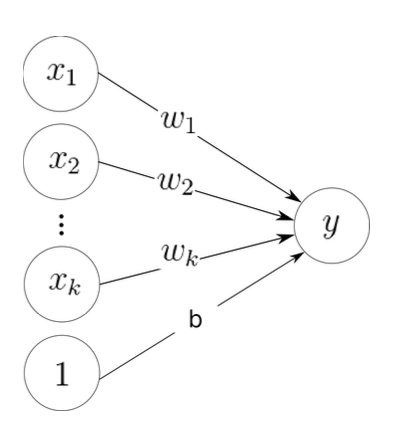
\includegraphics[width=.7\linewidth]{neuron.png}
		\captionof{figure}{The linear perceptron with single output}
		\label{fig:test1}
	\end{minipage}%
	~
	\begin{minipage}[c]{.49\textwidth}
		\centering
			\begin{tabular}{|c|c|c|c|}
				\hline
				$\overline{x}_{i,1}$ & $\overline{x}_{i,2}$ & $\overline{x}_{i,3}$ & $\hat{y}_i$ \\\hline
				-9         & -5         & 5          & 0                           \\\hline
				4          & -7         & -11        & 0                           \\\hline
				7          & 6          & -1         & 1                           \\\hline
				-9         & -5         & 4          & 1                           \\\hline
				-5         & -6         & -1         & 1                           \\\hline
				-4         & -4         & -8         & 0                           \\\hline
				5          & 7          & -9         & 1                           \\\hline
				2          & -4         & 3          & 0                           \\\hline
				-6         & 1          & 7          & 0                           \\\hline
				-10        & 6          & -7         & 1                          \\\hline
			\end{tabular}
			\captionof{table}{The training dataset}
			\label{tab:traind-dataset}
	
	\end{minipage}
\end{figure}

Before working on a neural network we will study the perceptron; a linear classifier
without an activation function or a very simple single layer network as given in Figure 1.
You are given a dataset of size $n: \mathcal{D} = \{(\overline{x}_1 ,\hat{y}_1),(\overline{x}_n ,\hat{y}_2),\dots , (\overline{x}_n ,\hat{y}_n)\}$, where input is represented as $k$-dimensional vectors $\overline{x}_i \in \mathbb{R}^k$, and the targets $\hat{y}_i \in \mathbb{R}$ are scalar. Assume bias term $b \in \mathbb{R}$ is not part of weight matrix $\underline{W} = [w_1,w_2,\dots,w_k]^T$.

\newpage

\Problem{What is the dimension of the output vector $\overline{y}$ if we assume a batch of input data in form $\underline{x} \in \mathbb{R}^{d \times k}$?}

\Solution{The output shape of the vector $\overline{y}$ is $d$. Given $d$ batch as input, the resulting output as the same dimension $d$.}

\Problem{Write down the vectorised equation for the forward pass, if input $\underline{x} \in \mathbb{R}^{d \times k}$ is batch of data, and $\overline{1}_d$ is a length $d$ long vector of ones (watch out for dimensions to match).}

\Solution{
	\begin{equation}
	\overline{y}=\sigma(\underline{x} \, \underline{W}+\overline{1}_d \, \overline{b}^T)
	\end{equation}
where:\begin{itemize}\itemsep-0.7em 
		\item[-] $\overline{y}$ is the output vector; \\
		\item[-] $\sigma$ is the activation function; \\
		\item[-] $\underline{x}$ is the input matrix; \\
		\item[-] $\underline{W}$ is the parameters matrix (weights); \\
		\item[-] $\overline{b}^T$ is the bias, that is a vector of $k$; \\
		\item[-] $\overline{1}_d$ is a vector  with $d$ ones, that is a vector of $k$.
\end{itemize}
For the specific exercise, the equation become:
	\begin{equation}
	\overline{y}=\underline{x} \, \underline{W}+\overline{1}_d \, b
	\end{equation}
	where $b$ is a single term and there isn't any activation function $\sigma$.
}

\Problem{Write down the vectorised equation for the MSE of the perceptron.}

\Solution{	
	\begin{equation}
	MSE = \frac{1}{2} \, (\overline{y}-\hat{\overline{y}})^T(\overline{y}-\hat{\overline{y}})
	\end{equation}}

\Problem{Determine the derivative of the error function w.r.t weights \textit{Hint: $\frac{\partial \overline{x}^T\overline{x}}{\partial\overline{x}^T} = 2\overline{x}$}}

\Solution{	
	\begin{equation}
	 \frac{\partial E}{\partial \underline{W}}= \frac{\partial \overline{y}}{\partial \underline{W}}\frac{\partial E}{\partial \overline{y}}
	\end{equation}
	Since the first factor is $\frac{\partial \overline{y}}{\partial \underline{W}}=\overline{x}^T$ and, using the given hint for the derivative of the inner product, the second factor become $\frac{\partial E}{\partial \overline{y}} = \frac{\partial }{\partial \overline{y}} \frac{1}{2}(\overline{y}-\hat{\overline{y}})^T(\overline{y}-\hat{\overline{y}}) = \frac{1}{2}2(\overline{y}-\hat{\overline{y}})=\overline{y}-\hat{\overline{y}}$
	
	 
	\begin{equation}
		 \frac{\partial E}{\partial \underline{W}}= \frac{\partial \overline{y}}{\partial \underline{W}}\frac{\partial E}{\partial \overline{y}} = \overline{x}^T(\overline{y}-\hat{\overline{y}})
	\end{equation}
}

\Problem{Write down the equation of the weight update by gradient descent.}

\Solution{	
	\begin{equation}
	\underline{W}^{\mathrm{NEW}}=\underline{W}^{\mathrm{OLD}}-\eta \frac{\partial E}{\partial \underline{W}}=\underline{W}^{\mathrm{OLD}}-\eta \, \overline{x}^T(\overline{y}-\hat{\overline{y}})
	\end{equation}
}

\Problem{Suppose $k = 3\mbox{, }d =10$, with a batch of data given in Table 1. The initial weights are $w_1 = -0.1$, $w_2 = -0.3$, $w_3 = 0.2$ and the bias weight is $b = 2$. Compute the weights after one step of gradient descent with learning rate of $\eta = 0.02$ (report their value up to 2 decimal points). \textit{Hint: MATLAB/Octave/Python might come in handy here.}}

\Solution{
	\begin{python}
		import numpy as np
				
		x = np.array([[ -9, -5,    5],
					   [   4, -7, -11],
					   [   7,   6,  -1],
					   [ -9, -5,    4],
					   [ -5, -6,  -1],
					   [ -4, -4,  -8],
					   [   5,   7,  -9],
					   [   2, -4,    3],
					   [ -6,   1,    7],
					   [-10,   6,  -7]],
					  dtype=np.float32)
		
		y_hat = np.array([0, 0, 1, 1, 1, 0, 1, 0, 0, 1], dtype=np.float32)
		W = np.array([-0.1, -0.3, 0.2], dtype=np.float32)
		b = 2
		eta = 0.02
		
		y = np.matmul(x, W) + b
		W_new = W - eta * np.matmul(np.transpose(x), (y - y_hat))
	\end{python}
	}

\Problem{Learning in multi-layer neural networks is usually done with help of two methods: back-propagation and gradient descent. Describe briefly what role in the learning process each of the two has (Should not be longer than $6$ lines).}

\Solution{Back-propagation  procedure (dynamic programming algorithm) for computing the gradient in an efficient way. In particular it consists in calculating the derivative of the error function with respect to the parameters (weights).\\
Gradient Descent is an algorithm that improve the models performance, decreasing the loss, updating the weights of the network by (using the) gradient (descent).}
\printbibliography
\nocite{*}

\end{document}




















